%=============================================================================
%   Configurations Found
%   Reporte de pentominos - Experiment Results
%   Servicio social - Laura Natalia Borbolla Palacios
%=============================================================================

\newpage
\subsection{Configurations found}
Below are presented the configurations that were found while observing the
evolutions of the pentominos; it is important to remark that, due to the
fast paced population growth in some pentominoes, it is possible that some
configurations remain hidden. The configurations are listed in the order that
were found.

\subsubsection{Gliders}

For more information, please consult \cite{j2}.

The gliders, as explained in section \ref{sec:brief_summary:cellular_automaton},
are mobile particles traveling in the space. There are two types of gliders:
primary and compound; the first ones cannot be decomposed into smaller mobile
localizations, whereas a compound glider is made of at least two primary
gliders. Some properties of the gliders are listed below:
\begin{itemize}
  \item Volume
  \item Translation
  \item Period
  \item Speed
  \item Weight
\end{itemize}

One of the primary gliders in the Diffusion Rule is shown in
figure~\ref{fig:dr-glider-1}.

\begin{figure}
	\centering
	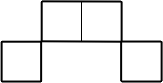
\includegraphics[scale=0.5]{df_settings_dd/dr-glider-1.png}
	\caption{G1 glider in the Diffusion Rule.}
  \label{fig:dr-glider-1}
\end{figure}

\paragraph{Glider-1}
Glider found in the evolutions of \ref{sec:p-pentomino}.
\begin{figure}
	\centering
	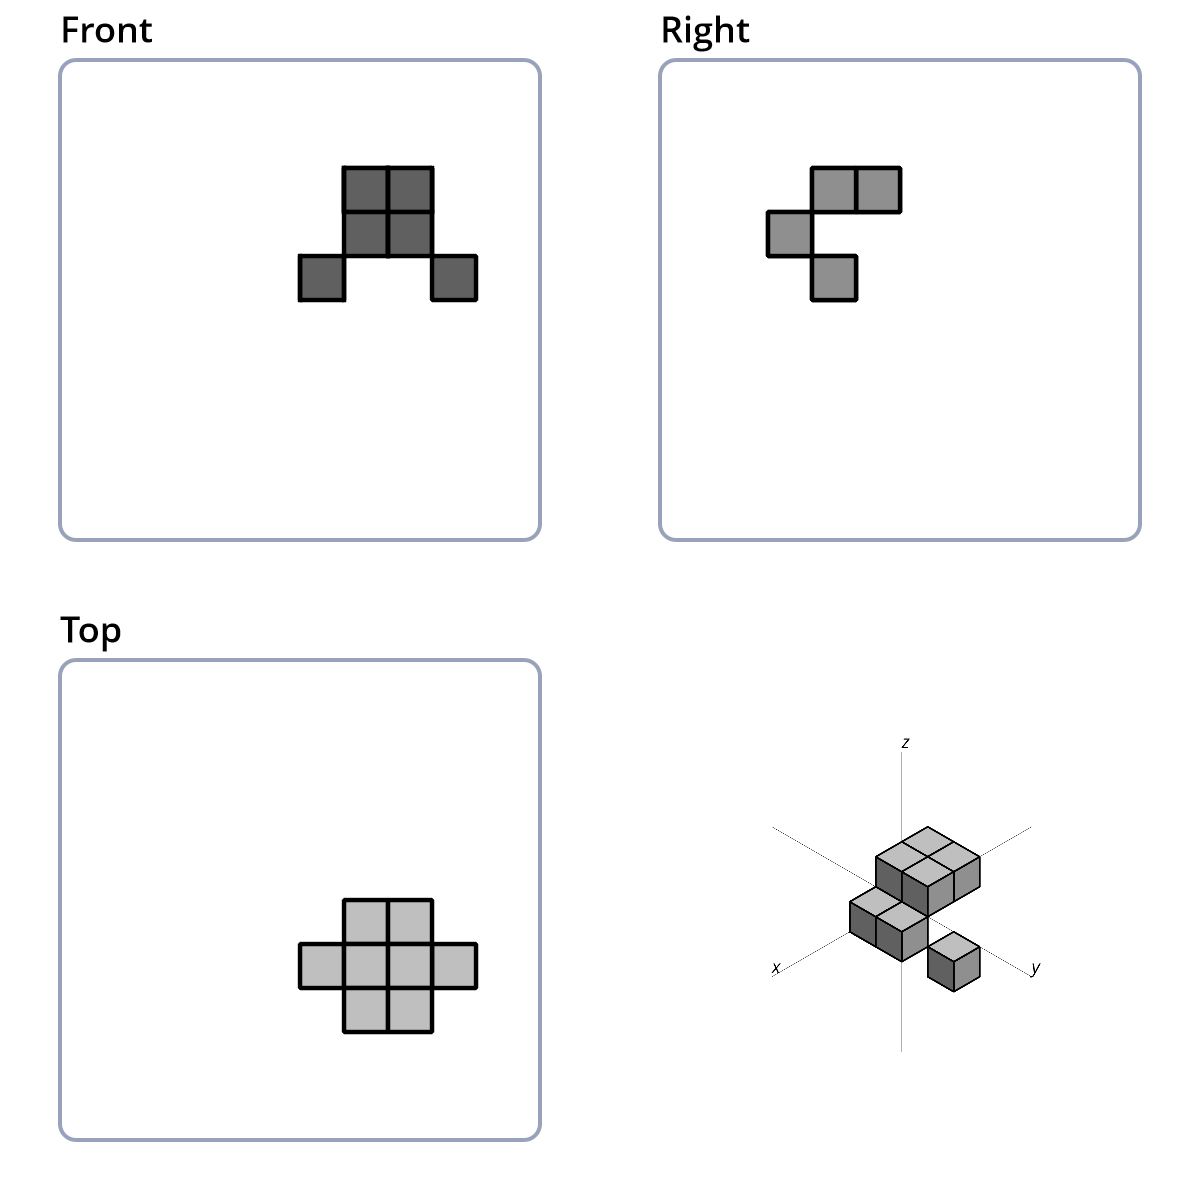
\includegraphics[scale=0.3]{iso_settings/glider_1.png}
	\caption{Isometric of glider-1.}
  \label{fig:iso-glider-1}
\end{figure}

\paragraph{Glider-2}
Glider found in the evolutions of \ref{sec:p-pentomino}.
\begin{figure}
	\centering
	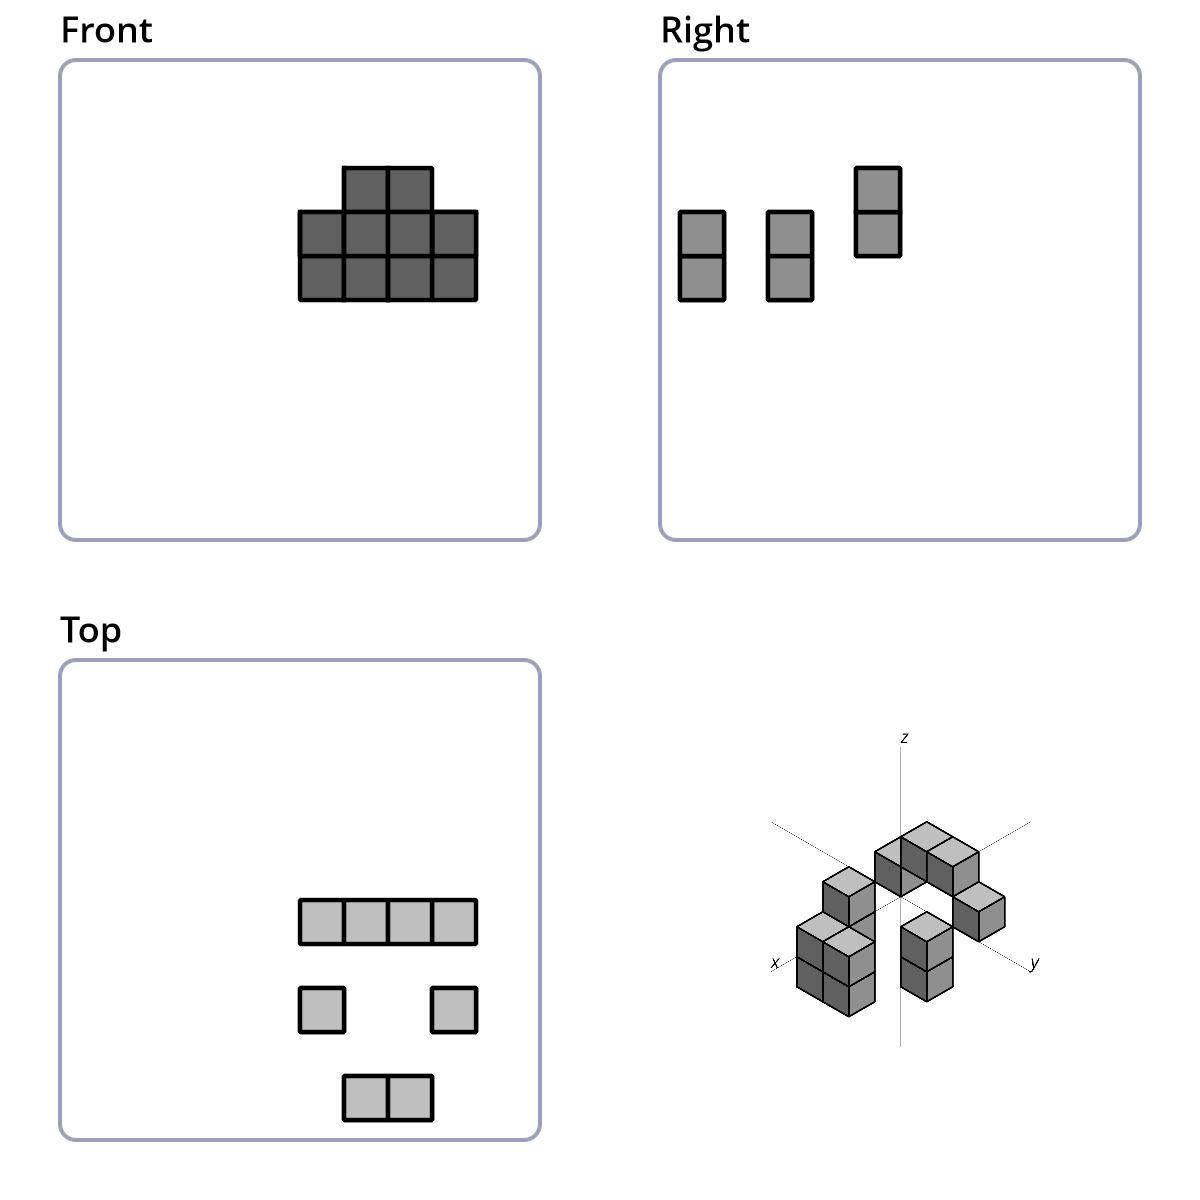
\includegraphics[scale=0.3]{iso_settings/glider_2.png}
	\caption{Isometric of glider-2.}
  \label{fig:iso-glider-2}
\end{figure}

\paragraph{Glider-3}
Glider found in the evolutions of \ref{sec:q-pentomino}.
\begin{figure}
  \centering
  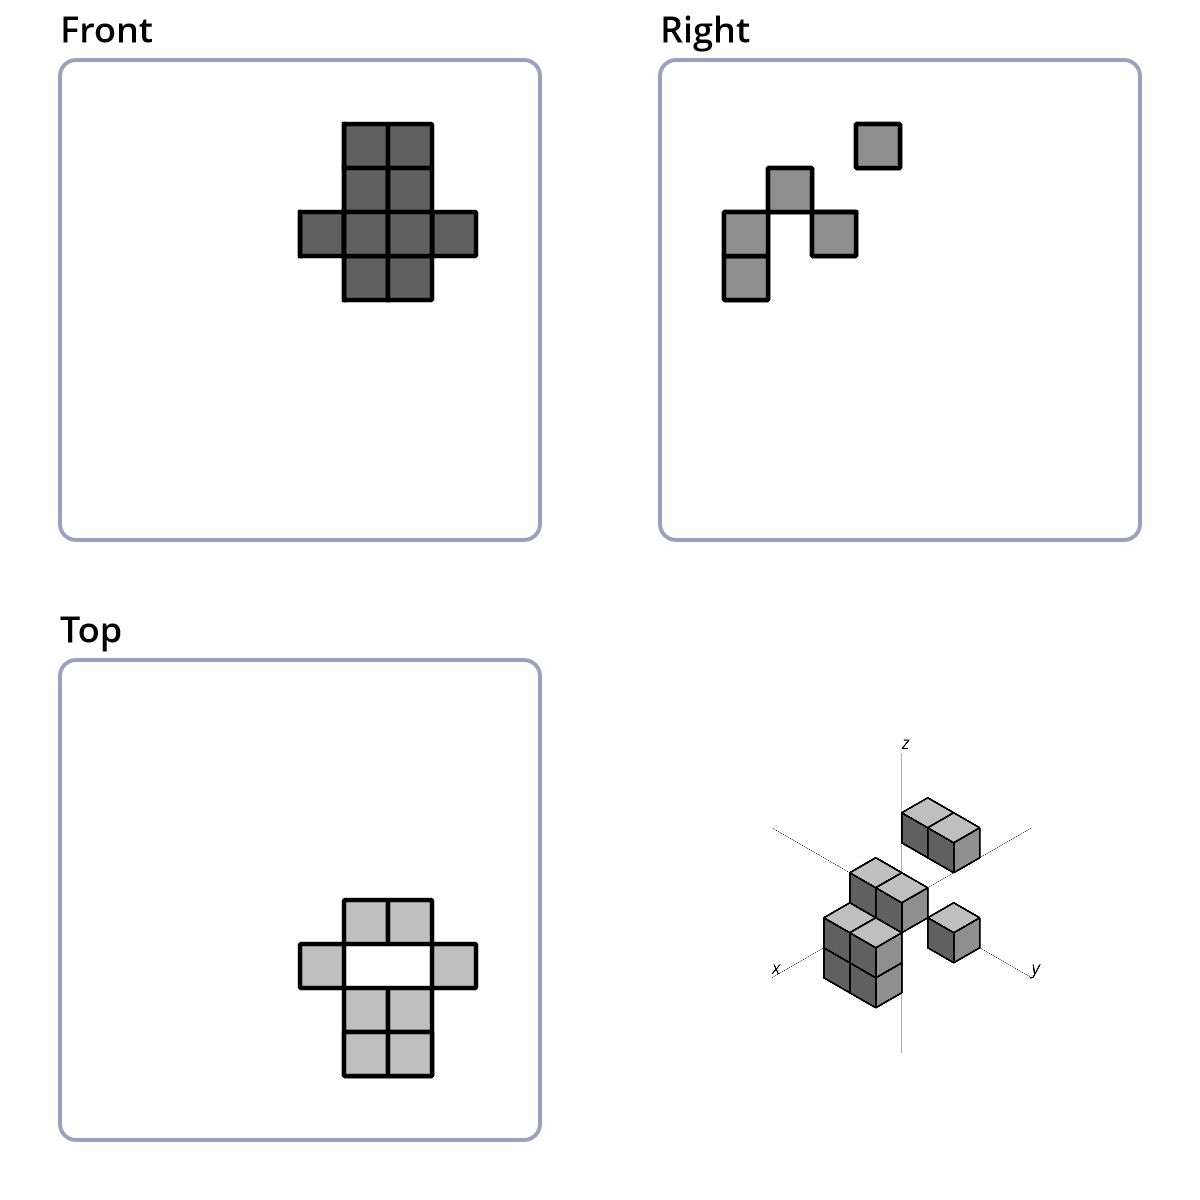
\includegraphics[scale=0.3]{iso_settings/glider_3.png}
  \caption{Isometric of glider-3.}
  \label{fig:iso-glider-3}
\end{figure}

\paragraph{Glider-4}
Glider found in the evolutions of \ref{sec:q-pentomino}.
This is, probably, the most simple glider; the equivalent
of~\ref{fig:dr-glider-1} in three dimensions.
\begin{figure}
  \centering
  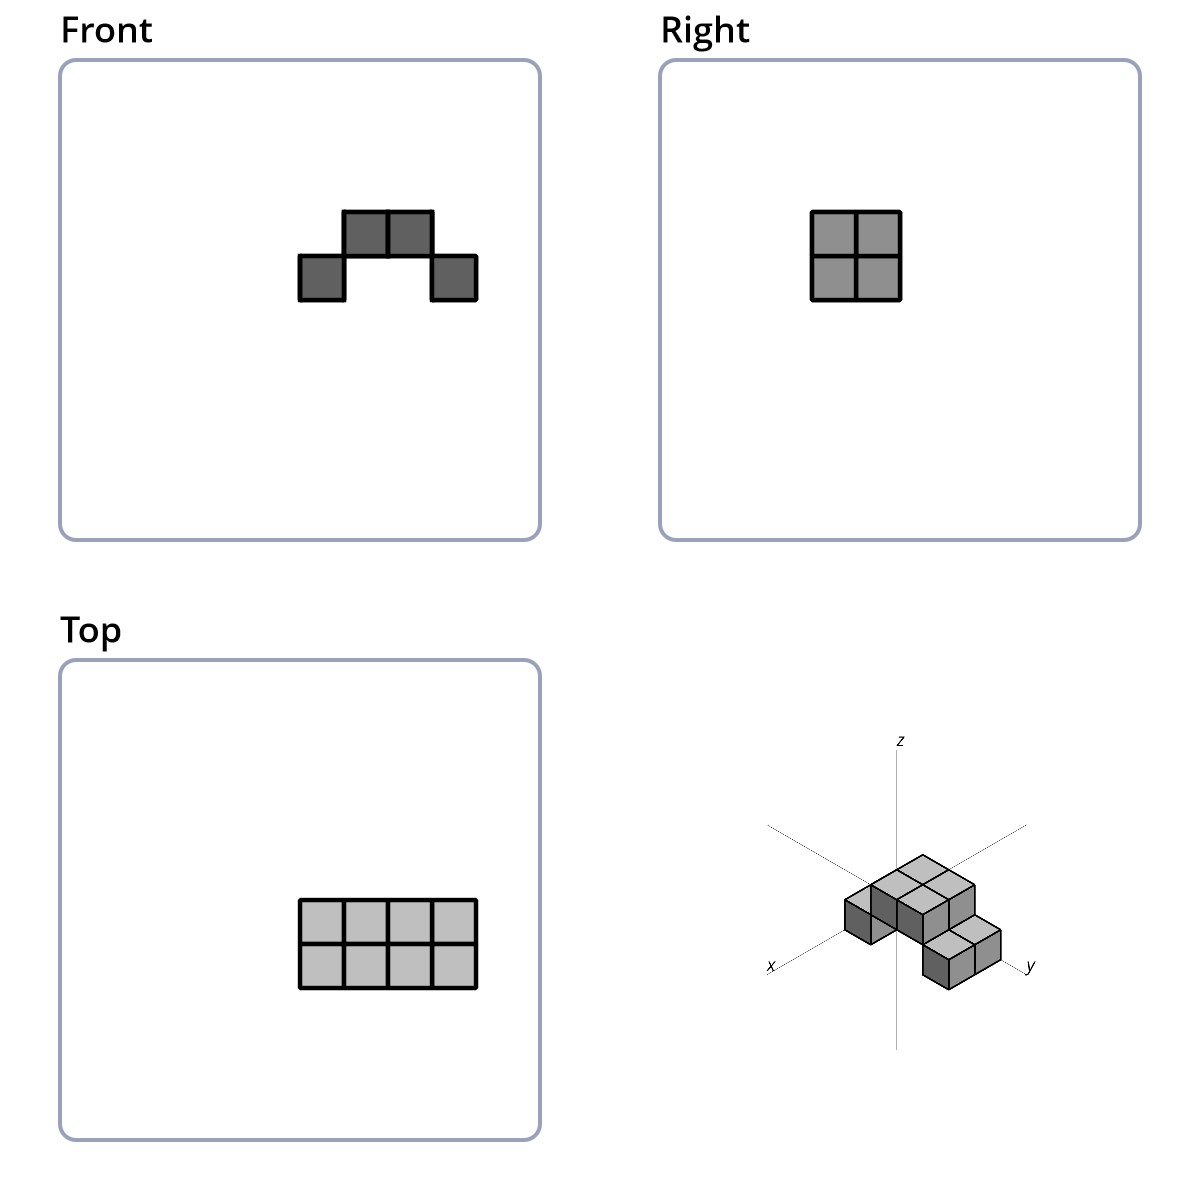
\includegraphics[scale=0.3]{iso_settings/glider_4.png}
  \caption{Isometric of glider-4.}
  \label{fig:iso-glider-4}
\end{figure}


\subsubsection{Oscillators}

\paragraph{Oscillator-1}
Oscillator found in the evolutions of~\ref{sec:o-pentomino}.

\begin{figure}
	\centering
	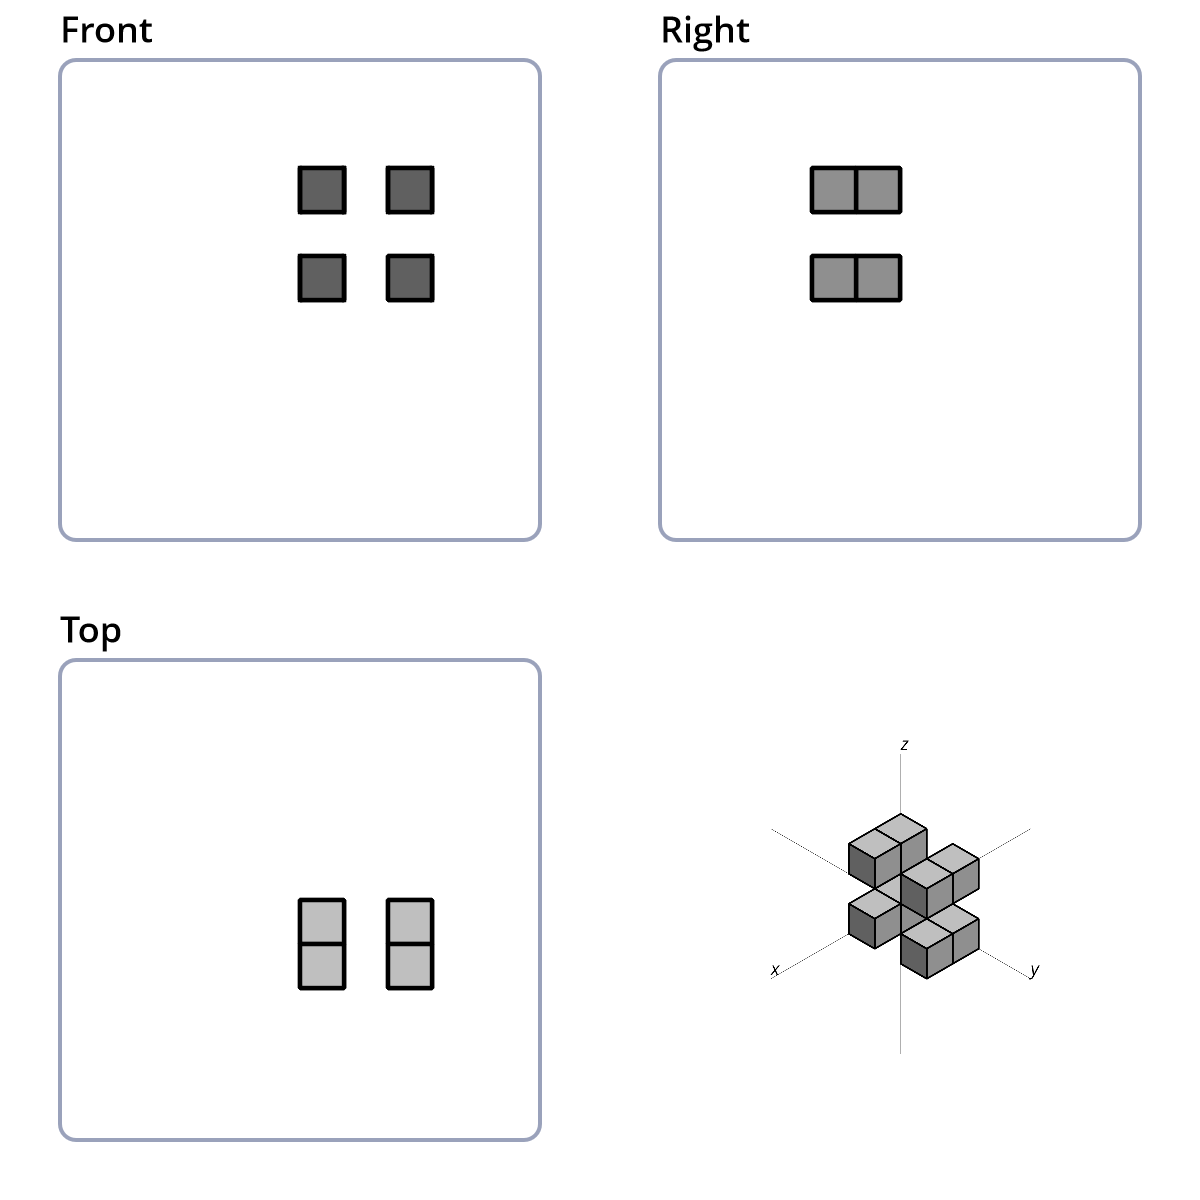
\includegraphics[scale=0.3]{iso_settings/osc_1.png}
	\caption{Isometric of oscillator-1.}
  \label{fig:iso-osc-1}
\end{figure}

\subsubsection{Puffer trains}
Oscilattor found in the evolutions of~\ref{sec:p-pentomino}.

\begin{figure}
	\centering
	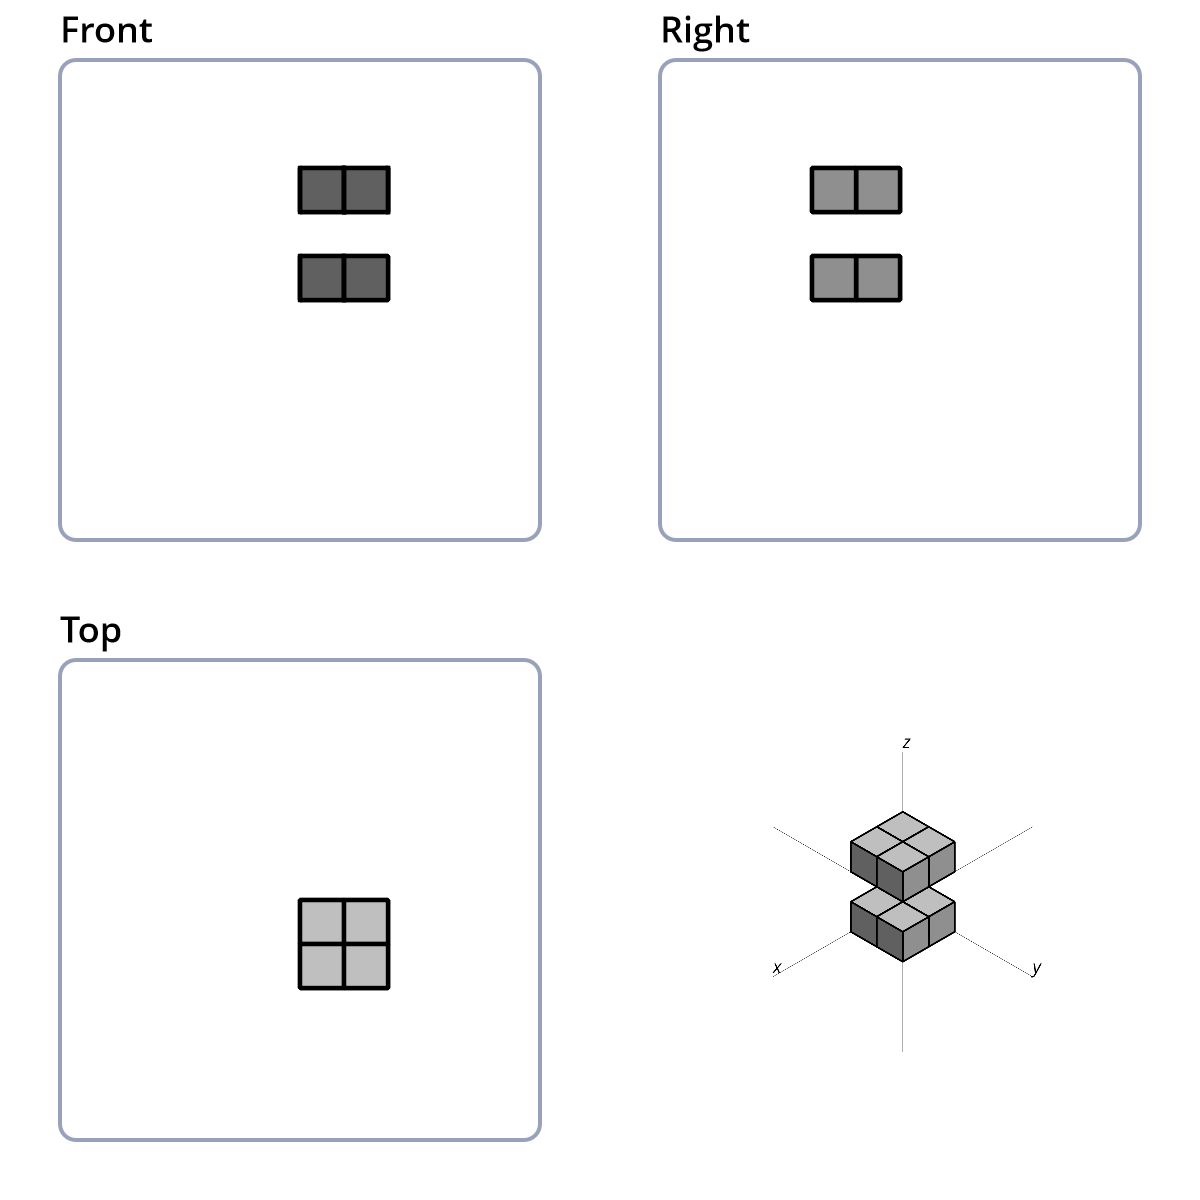
\includegraphics[scale=0.3]{iso_settings/puffer_1.png}
	\caption{Isometric of puffer-1.}
  \label{fig:iso-puffer-1}
\end{figure}
